\documentclass{article}
\usepackage{geometry}
 \geometry{
 a4paper,
 total={210mm,297mm},
 left=10mm,
 right=20mm,
 top=20mm,
 bottom=20mm,
 }
\usepackage{tikz}
\usetikzlibrary{mindmap,trees}
\tikzset{concept/.append style={fill={none}}}
\begin{document}
\pagestyle{empty}
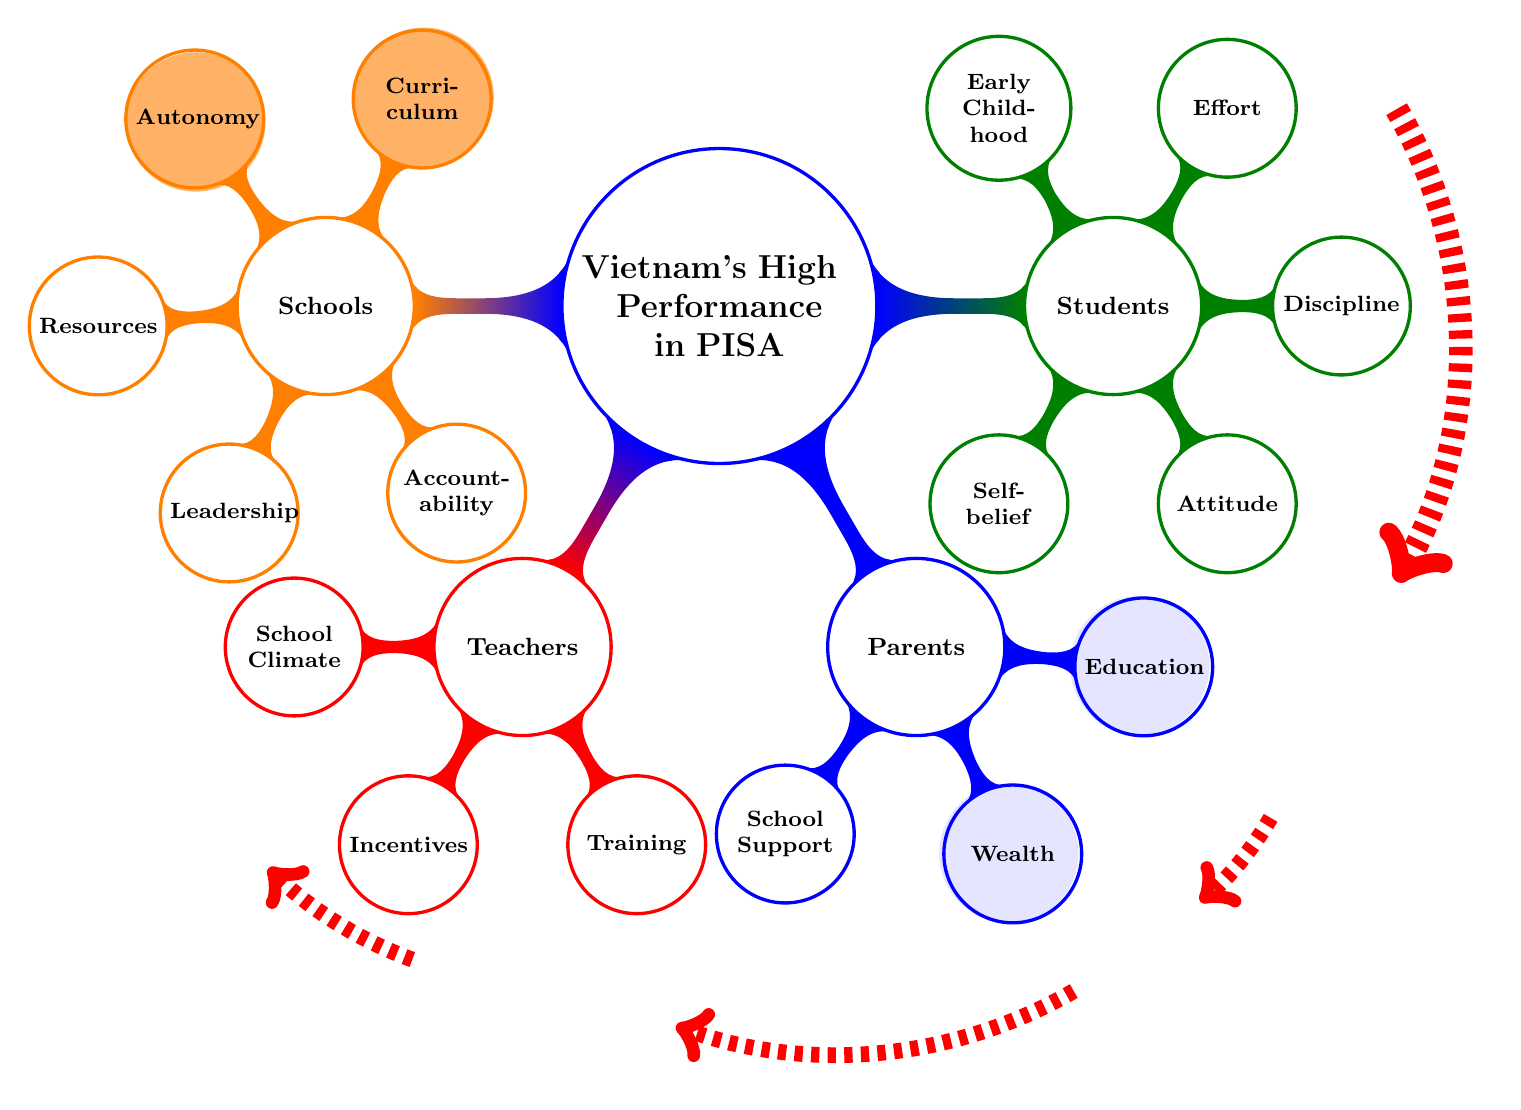
\begin{tikzpicture}[font=\sffamily\LARGE\bfseries]
        \path [fill=blue!10] (5.338,-4.568) circle [radius=0.885];
        \path [fill=blue!10] (3.675,-6.95) circle [radius=0.885];
        \path [fill=orange!60] (-6.65,2.338) circle [radius=0.885];
        \path [fill=orange!60] (-3.75,2.65) circle [radius=0.885];
     \path[mindmap,concept color=blue,text=black]
   node[concept] {\textbf{Vietnam's High \newline Performance in PISA}}
    [clockwise from=0]
      child[concept color=green!50!black] {
      node[concept] {\textbf{Students}}
      [clockwise from=120]
      child { node[concept] {\textbf{Early Childhood}}}
      child { node[concept] {\textbf{Effort}} }
      child { node[concept] { \textbf{Discipline}} }
      child { node[concept] {\textbf{Attitude}} }
      child { node[concept] {\textbf{Self-belief}} }
    }  
      child[concept color=blue] {
      node[concept] {\textbf{Parents}}
      [clockwise from=-5]
      child { node[concept] {\textbf{Education}} }
      child { node[concept] {\textbf{Wealth}} }
      child { node[concept] {\textbf{School Support}} }
    }
      child[concept color=red] { 
      node[concept] {\textbf{Teachers}} 
      [clockwise from=-60]
      child {node[concept] {\textbf{Training}}}
      child {node[concept] {\textbf{Incentives}}}
      child {node[concept] {\textbf{School Climate}}}
      }
      child[concept color=orange] {
      node[concept] {\textbf{Schools}} 
      [clockwise from=-55]
      child {node[concept] {\textbf{Account- ability}}}
      child {node[concept] {\textbf{Leadership}}} 
      child {node[concept] {\textbf{Resources}}}      
      child {node[concept] {\textbf{Autonomy}}}      
      child {node[concept] {\textbf{Curri- culum}}} 
      };
    \draw [line width=0.3cm, ->, dashed, red](8.6,2.5) arc 
    [radius=6, start angle=30, end angle= -30];
       \draw [line width=0.2cm, ->, dashed, red](7,-6.5) arc [radius=4cm, start angle=-30, end angle= -50];
        \draw [line width=0.2cm, ->, dashed, red](4.5,-8.7) arc [radius=6cm, start angle=-60, end angle= -110];
         \draw [line width=0.2cm, ->, dashed, red](-3.9,-8.3) arc [radius=5cm, start angle=-110, end angle= -135];
             %\draw [line width=0.2cm, ->, dashed, red](-9.3,-2.8) arc [radius=5cm, start angle=-165, end angle= -185];
         \end{tikzpicture}
\end{document}